\documentclass[]{article}
\usepackage{lmodern}
\usepackage{amssymb,amsmath}
\usepackage{ifxetex,ifluatex}
\usepackage{fixltx2e} % provides \textsubscript
\ifnum 0\ifxetex 1\fi\ifluatex 1\fi=0 % if pdftex
  \usepackage[T1]{fontenc}
  \usepackage[utf8]{inputenc}
\else % if luatex or xelatex
  \ifxetex
    \usepackage{mathspec}
  \else
    \usepackage{fontspec}
  \fi
  \defaultfontfeatures{Ligatures=TeX,Scale=MatchLowercase}
\fi
% use upquote if available, for straight quotes in verbatim environments
\IfFileExists{upquote.sty}{\usepackage{upquote}}{}
% use microtype if available
\IfFileExists{microtype.sty}{%
\usepackage{microtype}
\UseMicrotypeSet[protrusion]{basicmath} % disable protrusion for tt fonts
}{}
\usepackage[margin=1in]{geometry}
\usepackage{hyperref}
\hypersetup{unicode=true,
            pdftitle={Data\_setup},
            pdfauthor={Rachel Schattman},
            pdfborder={0 0 0},
            breaklinks=true}
\urlstyle{same}  % don't use monospace font for urls
\usepackage{color}
\usepackage{fancyvrb}
\newcommand{\VerbBar}{|}
\newcommand{\VERB}{\Verb[commandchars=\\\{\}]}
\DefineVerbatimEnvironment{Highlighting}{Verbatim}{commandchars=\\\{\}}
% Add ',fontsize=\small' for more characters per line
\usepackage{framed}
\definecolor{shadecolor}{RGB}{248,248,248}
\newenvironment{Shaded}{\begin{snugshade}}{\end{snugshade}}
\newcommand{\KeywordTok}[1]{\textcolor[rgb]{0.13,0.29,0.53}{\textbf{{#1}}}}
\newcommand{\DataTypeTok}[1]{\textcolor[rgb]{0.13,0.29,0.53}{{#1}}}
\newcommand{\DecValTok}[1]{\textcolor[rgb]{0.00,0.00,0.81}{{#1}}}
\newcommand{\BaseNTok}[1]{\textcolor[rgb]{0.00,0.00,0.81}{{#1}}}
\newcommand{\FloatTok}[1]{\textcolor[rgb]{0.00,0.00,0.81}{{#1}}}
\newcommand{\ConstantTok}[1]{\textcolor[rgb]{0.00,0.00,0.00}{{#1}}}
\newcommand{\CharTok}[1]{\textcolor[rgb]{0.31,0.60,0.02}{{#1}}}
\newcommand{\SpecialCharTok}[1]{\textcolor[rgb]{0.00,0.00,0.00}{{#1}}}
\newcommand{\StringTok}[1]{\textcolor[rgb]{0.31,0.60,0.02}{{#1}}}
\newcommand{\VerbatimStringTok}[1]{\textcolor[rgb]{0.31,0.60,0.02}{{#1}}}
\newcommand{\SpecialStringTok}[1]{\textcolor[rgb]{0.31,0.60,0.02}{{#1}}}
\newcommand{\ImportTok}[1]{{#1}}
\newcommand{\CommentTok}[1]{\textcolor[rgb]{0.56,0.35,0.01}{\textit{{#1}}}}
\newcommand{\DocumentationTok}[1]{\textcolor[rgb]{0.56,0.35,0.01}{\textbf{\textit{{#1}}}}}
\newcommand{\AnnotationTok}[1]{\textcolor[rgb]{0.56,0.35,0.01}{\textbf{\textit{{#1}}}}}
\newcommand{\CommentVarTok}[1]{\textcolor[rgb]{0.56,0.35,0.01}{\textbf{\textit{{#1}}}}}
\newcommand{\OtherTok}[1]{\textcolor[rgb]{0.56,0.35,0.01}{{#1}}}
\newcommand{\FunctionTok}[1]{\textcolor[rgb]{0.00,0.00,0.00}{{#1}}}
\newcommand{\VariableTok}[1]{\textcolor[rgb]{0.00,0.00,0.00}{{#1}}}
\newcommand{\ControlFlowTok}[1]{\textcolor[rgb]{0.13,0.29,0.53}{\textbf{{#1}}}}
\newcommand{\OperatorTok}[1]{\textcolor[rgb]{0.81,0.36,0.00}{\textbf{{#1}}}}
\newcommand{\BuiltInTok}[1]{{#1}}
\newcommand{\ExtensionTok}[1]{{#1}}
\newcommand{\PreprocessorTok}[1]{\textcolor[rgb]{0.56,0.35,0.01}{\textit{{#1}}}}
\newcommand{\AttributeTok}[1]{\textcolor[rgb]{0.77,0.63,0.00}{{#1}}}
\newcommand{\RegionMarkerTok}[1]{{#1}}
\newcommand{\InformationTok}[1]{\textcolor[rgb]{0.56,0.35,0.01}{\textbf{\textit{{#1}}}}}
\newcommand{\WarningTok}[1]{\textcolor[rgb]{0.56,0.35,0.01}{\textbf{\textit{{#1}}}}}
\newcommand{\AlertTok}[1]{\textcolor[rgb]{0.94,0.16,0.16}{{#1}}}
\newcommand{\ErrorTok}[1]{\textcolor[rgb]{0.64,0.00,0.00}{\textbf{{#1}}}}
\newcommand{\NormalTok}[1]{{#1}}
\usepackage{graphicx,grffile}
\makeatletter
\def\maxwidth{\ifdim\Gin@nat@width>\linewidth\linewidth\else\Gin@nat@width\fi}
\def\maxheight{\ifdim\Gin@nat@height>\textheight\textheight\else\Gin@nat@height\fi}
\makeatother
% Scale images if necessary, so that they will not overflow the page
% margins by default, and it is still possible to overwrite the defaults
% using explicit options in \includegraphics[width, height, ...]{}
\setkeys{Gin}{width=\maxwidth,height=\maxheight,keepaspectratio}
\IfFileExists{parskip.sty}{%
\usepackage{parskip}
}{% else
\setlength{\parindent}{0pt}
\setlength{\parskip}{6pt plus 2pt minus 1pt}
}
\setlength{\emergencystretch}{3em}  % prevent overfull lines
\providecommand{\tightlist}{%
  \setlength{\itemsep}{0pt}\setlength{\parskip}{0pt}}
\setcounter{secnumdepth}{0}
% Redefines (sub)paragraphs to behave more like sections
\ifx\paragraph\undefined\else
\let\oldparagraph\paragraph
\renewcommand{\paragraph}[1]{\oldparagraph{#1}\mbox{}}
\fi
\ifx\subparagraph\undefined\else
\let\oldsubparagraph\subparagraph
\renewcommand{\subparagraph}[1]{\oldsubparagraph{#1}\mbox{}}
\fi

%%% Use protect on footnotes to avoid problems with footnotes in titles
\let\rmarkdownfootnote\footnote%
\def\footnote{\protect\rmarkdownfootnote}

%%% Change title format to be more compact
\usepackage{titling}

% Create subtitle command for use in maketitle
\providecommand{\subtitle}[1]{
  \posttitle{
    \begin{center}\large#1\end{center}
    }
}

\setlength{\droptitle}{-2em}

  \title{Data\_setup}
    \pretitle{\vspace{\droptitle}\centering\huge}
  \posttitle{\par}
    \author{Rachel Schattman}
    \preauthor{\centering\large\emph}
  \postauthor{\par}
      \predate{\centering\large\emph}
  \postdate{\par}
    \date{February 19, 2019}


\begin{document}
\maketitle

\section{load libraries}\label{load-libraries}

\begin{verbatim}
## 
## Attaching package: 'dplyr'
\end{verbatim}

\begin{verbatim}
## The following objects are masked from 'package:stats':
## 
##     filter, lag
\end{verbatim}

\begin{verbatim}
## The following objects are masked from 'package:base':
## 
##     intersect, setdiff, setequal, union
\end{verbatim}

\begin{verbatim}
## -------------------------------------------------------------------------
\end{verbatim}

\begin{verbatim}
## You have loaded plyr after dplyr - this is likely to cause problems.
## If you need functions from both plyr and dplyr, please load plyr first, then dplyr:
## library(plyr); library(dplyr)
\end{verbatim}

\begin{verbatim}
## -------------------------------------------------------------------------
\end{verbatim}

\begin{verbatim}
## 
## Attaching package: 'plyr'
\end{verbatim}

\begin{verbatim}
## The following objects are masked from 'package:dplyr':
## 
##     arrange, count, desc, failwith, id, mutate, rename, summarise,
##     summarize
\end{verbatim}

\begin{verbatim}
## Warning: package 'randomForest' was built under R version 3.5.3
\end{verbatim}

\begin{verbatim}
## randomForest 4.6-14
\end{verbatim}

\begin{verbatim}
## Type rfNews() to see new features/changes/bug fixes.
\end{verbatim}

\begin{verbatim}
## 
## Attaching package: 'randomForest'
\end{verbatim}

\begin{verbatim}
## The following object is masked from 'package:dplyr':
## 
##     combine
\end{verbatim}

\begin{verbatim}
## Warning: package 'Metrics' was built under R version 3.5.3
\end{verbatim}

\section{Helpful resources:}\label{helpful-resources}

\subsection{\texorpdfstring{\url{https://www.r-bloggers.com/how-to-implement-random-forests-in-r/}}{https://www.r-bloggers.com/how-to-implement-random-forests-in-r/}}\label{httpswww.r-bloggers.comhow-to-implement-random-forests-in-r}

\subsection{\texorpdfstring{\url{https://cran.r-project.org/web/packages/randomForest/randomForest.pdf}}{https://cran.r-project.org/web/packages/randomForest/randomForest.pdf}}\label{httpscran.r-project.orgwebpackagesrandomforestrandomforest.pdf}

\subsection{\texorpdfstring{\url{https://rpubs.com/mbaumer/randomForest}}{https://rpubs.com/mbaumer/randomForest}}\label{httpsrpubs.commbaumerrandomforest}

\begin{Shaded}
\begin{Highlighting}[]
\NormalTok{script_path <-}\StringTok{ "C:/Users/rschattman/Documents/Research/RandomForestRMA/data"}
\NormalTok{in_dir <-}\StringTok{ "C:/Users/rschattman/Documents/Research/RandomForestRMA/data"}
\NormalTok{out_dir <-}\StringTok{ "C:/Users/rschattman/Documents/Research/RandomForestRMA/output/data"}
\end{Highlighting}
\end{Shaded}

\section{Read in data and combine into single
dataframe}\label{read-in-data-and-combine-into-single-dataframe}

\begin{Shaded}
\begin{Highlighting}[]
\NormalTok{PAcip <-}\StringTok{ }\KeywordTok{read.csv}\NormalTok{(}\DataTypeTok{file =} \StringTok{"C:/Users/rschattman/Documents/Research/RandomForestRMA/data/monthly_prcp_PA.csv"}\NormalTok{, }\DataTypeTok{header =} \OtherTok{TRUE}\NormalTok{, }\DataTypeTok{sep =} \StringTok{","}\NormalTok{)}
\NormalTok{PAloss <-}\StringTok{ }\KeywordTok{read.csv}\NormalTok{(}\DataTypeTok{file =} \StringTok{"C:/Users/rschattman/Documents/Research/RandomForestRMA/data/PAannuallosses.csv"}\NormalTok{, }\DataTypeTok{header =} \OtherTok{TRUE}\NormalTok{, }\DataTypeTok{sep =} \StringTok{","}\NormalTok{)}
\NormalTok{PAbeta <-}\KeywordTok{merge}\NormalTok{(PAcip, PAloss)}
\end{Highlighting}
\end{Shaded}

\section{Create new data frames with one dependent
variable}\label{create-new-data-frames-with-one-dependent-variable}

\begin{Shaded}
\begin{Highlighting}[]
\KeywordTok{head}\NormalTok{(PAbeta)}
\end{Highlighting}
\end{Shaded}

\begin{verbatim}
##   Year month StateCollege_PRCP Lebanon_PRCP Selinsgrove_PRCP State
## 1 2001     1              3.39         6.69             3.71    PA
## 2 2001     2              1.87         4.08             2.85    PA
## 3 2001     3             10.70         8.51            12.10    PA
## 4 2001     4              6.75         6.93             5.65    PA
## 5 2001     5              3.51         9.61             4.78    PA
## 6 2001     6             12.76         6.79            16.53    PA
##   WetDollars WetAcres nWet DryDollars DryAcres nDry
## 1     129986  1700.12   57   14721696   216408  478
## 2     129986  1700.12   57   14721696   216408  478
## 3     129986  1700.12   57   14721696   216408  478
## 4     129986  1700.12   57   14721696   216408  478
## 5     129986  1700.12   57   14721696   216408  478
## 6     129986  1700.12   57   14721696   216408  478
\end{verbatim}

\begin{Shaded}
\begin{Highlighting}[]
\NormalTok{WetAcres <-}\StringTok{ }\NormalTok{PAbeta[,}\KeywordTok{c}\NormalTok{(}\StringTok{"Year"}\NormalTok{, }\StringTok{"month"}\NormalTok{, }\StringTok{"StateCollege_PRCP"}\NormalTok{, }\StringTok{"Lebanon_PRCP"}\NormalTok{, }\StringTok{"Selinsgrove_PRCP"}\NormalTok{, }\StringTok{"WetAcres"}\NormalTok{)]}
\NormalTok{WetDollars <-}\StringTok{ }\NormalTok{PAbeta[,}\KeywordTok{c}\NormalTok{(}\StringTok{"Year"}\NormalTok{, }\StringTok{"month"}\NormalTok{, }\StringTok{"StateCollege_PRCP"}\NormalTok{, }\StringTok{"Lebanon_PRCP"}\NormalTok{, }\StringTok{"Selinsgrove_PRCP"}\NormalTok{, }\StringTok{"WetDollars"}\NormalTok{)]}
\NormalTok{DryDollars <-}\StringTok{ }\NormalTok{PAbeta[,}\KeywordTok{c}\NormalTok{(}\StringTok{"Year"}\NormalTok{, }\StringTok{"month"}\NormalTok{, }\StringTok{"StateCollege_PRCP"}\NormalTok{, }\StringTok{"Lebanon_PRCP"}\NormalTok{, }\StringTok{"Selinsgrove_PRCP"}\NormalTok{, }\StringTok{"DryDollars"}\NormalTok{)]}
\NormalTok{DryAcres <-}\StringTok{ }\NormalTok{PAbeta[,}\KeywordTok{c}\NormalTok{(}\StringTok{"Year"}\NormalTok{, }\StringTok{"month"}\NormalTok{, }\StringTok{"StateCollege_PRCP"}\NormalTok{, }\StringTok{"Lebanon_PRCP"}\NormalTok{, }\StringTok{"Selinsgrove_PRCP"}\NormalTok{, }\StringTok{"DryAcres"}\NormalTok{)]}
\end{Highlighting}
\end{Shaded}

\section{Review data}\label{review-data}

\begin{Shaded}
\begin{Highlighting}[]
\KeywordTok{head}\NormalTok{(WetAcres)}
\end{Highlighting}
\end{Shaded}

\begin{verbatim}
##   Year month StateCollege_PRCP Lebanon_PRCP Selinsgrove_PRCP WetAcres
## 1 2001     1              3.39         6.69             3.71  1700.12
## 2 2001     2              1.87         4.08             2.85  1700.12
## 3 2001     3             10.70         8.51            12.10  1700.12
## 4 2001     4              6.75         6.93             5.65  1700.12
## 5 2001     5              3.51         9.61             4.78  1700.12
## 6 2001     6             12.76         6.79            16.53  1700.12
\end{verbatim}

\begin{Shaded}
\begin{Highlighting}[]
\KeywordTok{str}\NormalTok{(WetAcres)}
\end{Highlighting}
\end{Shaded}

\begin{verbatim}
## 'data.frame':    216 obs. of  6 variables:
##  $ Year             : int  2001 2001 2001 2001 2001 2001 2001 2001 2001 2001 ...
##  $ month            : int  1 2 3 4 5 6 7 8 9 10 ...
##  $ StateCollege_PRCP: num  3.39 1.87 10.7 6.75 3.51 ...
##  $ Lebanon_PRCP     : num  6.69 4.08 8.51 6.93 9.61 ...
##  $ Selinsgrove_PRCP : num  3.71 2.85 12.1 5.65 4.78 ...
##  $ WetAcres         : num  1700 1700 1700 1700 1700 ...
\end{verbatim}

\begin{Shaded}
\begin{Highlighting}[]
\KeywordTok{summary}\NormalTok{(WetAcres)}
\end{Highlighting}
\end{Shaded}

\begin{verbatim}
##       Year          month       StateCollege_PRCP  Lebanon_PRCP   
##  Min.   :2001   Min.   : 1.00   Min.   : 1.560    Min.   : 0.910  
##  1st Qu.:2005   1st Qu.: 3.75   1st Qu.: 5.495    1st Qu.: 6.295  
##  Median :2010   Median : 6.50   Median : 8.065    Median : 9.555  
##  Mean   :2010   Mean   : 6.50   Mean   : 8.953    Mean   :10.134  
##  3rd Qu.:2014   3rd Qu.: 9.25   3rd Qu.:11.445    3rd Qu.:12.307  
##  Max.   :2018   Max.   :12.00   Max.   :26.840    Max.   :45.690  
##  Selinsgrove_PRCP    WetAcres     
##  Min.   : 0.000   Min.   :  1700  
##  1st Qu.: 5.420   1st Qu.:  8658  
##  Median : 7.985   Median : 54857  
##  Mean   : 9.064   Mean   : 61888  
##  3rd Qu.:11.810   3rd Qu.: 98898  
##  Max.   :48.100   Max.   :221234
\end{verbatim}

\section{Split into trainning, validation, and test
sets}\label{split-into-trainning-validation-and-test-sets}

\begin{Shaded}
\begin{Highlighting}[]
\KeywordTok{set.seed}\NormalTok{(}\DecValTok{25}\NormalTok{)}
\NormalTok{assignment <-}\StringTok{ }\KeywordTok{sample}\NormalTok{(}\DecValTok{1}\NormalTok{:}\DecValTok{3}\NormalTok{, }\DataTypeTok{size =} \KeywordTok{nrow}\NormalTok{(WetAcres), }\DataTypeTok{prob =} \KeywordTok{c}\NormalTok{(}\FloatTok{0.7}\NormalTok{, }\FloatTok{0.15}\NormalTok{, }\FloatTok{0.15}\NormalTok{), }\DataTypeTok{replace =} \OtherTok{TRUE}\NormalTok{)}

\NormalTok{Wettrain <-}\StringTok{ }\NormalTok{WetAcres[assignment ==}\StringTok{ }\DecValTok{1}\NormalTok{,]}
\NormalTok{Wetvalid <-}\StringTok{ }\NormalTok{WetAcres[assignment ==}\StringTok{ }\DecValTok{2}\NormalTok{,]}
\NormalTok{Wettest <-}\StringTok{ }\NormalTok{WetAcres[assignment ==}\StringTok{ }\DecValTok{3}\NormalTok{,]}

\KeywordTok{summary}\NormalTok{(Wettrain)}
\end{Highlighting}
\end{Shaded}

\begin{verbatim}
##       Year          month        StateCollege_PRCP  Lebanon_PRCP   
##  Min.   :2001   Min.   : 1.000   Min.   : 1.620    Min.   : 0.910  
##  1st Qu.:2005   1st Qu.: 4.000   1st Qu.: 5.270    1st Qu.: 6.335  
##  Median :2009   Median : 7.000   Median : 8.050    Median : 9.330  
##  Mean   :2009   Mean   : 6.638   Mean   : 8.831    Mean   : 9.718  
##  3rd Qu.:2014   3rd Qu.:10.000   3rd Qu.:11.370    3rd Qu.:12.145  
##  Max.   :2018   Max.   :12.000   Max.   :26.840    Max.   :39.150  
##  Selinsgrove_PRCP    WetAcres     
##  Min.   : 2.060   Min.   :  1700  
##  1st Qu.: 5.400   1st Qu.:  8658  
##  Median : 7.920   Median : 53338  
##  Mean   : 8.842   Mean   : 60893  
##  3rd Qu.:11.660   3rd Qu.: 98898  
##  Max.   :32.740   Max.   :221234
\end{verbatim}

\begin{Shaded}
\begin{Highlighting}[]
\KeywordTok{summary}\NormalTok{(Wetvalid)}
\end{Highlighting}
\end{Shaded}

\begin{verbatim}
##       Year          month        StateCollege_PRCP  Lebanon_PRCP   
##  Min.   :2001   Min.   : 1.000   Min.   : 1.56     Min.   : 1.190  
##  1st Qu.:2007   1st Qu.: 3.000   1st Qu.: 5.99     1st Qu.: 5.692  
##  Median :2012   Median : 6.000   Median : 7.82     Median : 9.090  
##  Mean   :2011   Mean   : 6.077   Mean   : 9.17     Mean   :11.616  
##  3rd Qu.:2015   3rd Qu.: 9.000   3rd Qu.:12.43     3rd Qu.:15.155  
##  Max.   :2018   Max.   :12.000   Max.   :22.57     Max.   :45.690  
##  Selinsgrove_PRCP    WetAcres     
##  Min.   : 0.000   Min.   :  1700  
##  1st Qu.: 5.675   1st Qu.: 12630  
##  Median : 8.850   Median : 54857  
##  Mean   :10.449   Mean   : 61611  
##  3rd Qu.:12.215   3rd Qu.:100669  
##  Max.   :48.100   Max.   :159070
\end{verbatim}

\begin{Shaded}
\begin{Highlighting}[]
\KeywordTok{summary}\NormalTok{(Wettest)}
\end{Highlighting}
\end{Shaded}

\begin{verbatim}
##       Year          month        StateCollege_PRCP  Lebanon_PRCP  
##  Min.   :2002   Min.   : 1.000   Min.   : 2.940    Min.   : 2.31  
##  1st Qu.:2004   1st Qu.: 4.000   1st Qu.: 6.495    1st Qu.: 6.39  
##  Median :2008   Median : 6.000   Median : 9.260    Median :10.04  
##  Mean   :2009   Mean   : 6.074   Mean   : 9.480    Mean   :11.22  
##  3rd Qu.:2014   3rd Qu.: 8.000   3rd Qu.:10.905    3rd Qu.:12.82  
##  Max.   :2018   Max.   :12.000   Max.   :19.730    Max.   :33.07  
##  Selinsgrove_PRCP    WetAcres     
##  Min.   : 0.200   Min.   :  5455  
##  1st Qu.: 5.165   1st Qu.: 12639  
##  Median : 8.960   Median : 56377  
##  Mean   : 9.075   Mean   : 68160  
##  3rd Qu.:11.850   3rd Qu.: 98898  
##  Max.   :26.700   Max.   :221234
\end{verbatim}

\section{Create Random Forest Model and test performance
metrics}\label{create-random-forest-model-and-test-performance-metrics}

\subsection{Wet Acres}\label{wet-acres}

\begin{Shaded}
\begin{Highlighting}[]
\NormalTok{Mod1 <-}\StringTok{ }\KeywordTok{randomForest}\NormalTok{(WetAcres ~}\StringTok{ }\NormalTok{., }
                     \DataTypeTok{data =} \NormalTok{Wettrain, }
                     \DataTypeTok{ntree =} \DecValTok{500}\NormalTok{, }
                     \CommentTok{#method = "anova", }
                     \DataTypeTok{importance =} \OtherTok{TRUE}\NormalTok{)}

\KeywordTok{print}\NormalTok{(Mod1)                                 }\CommentTok{# % of variance expalined is low. Tuning needed}
\end{Highlighting}
\end{Shaded}

\begin{verbatim}
## 
## Call:
##  randomForest(formula = WetAcres ~ ., data = Wettrain, ntree = 500,      importance = TRUE) 
##                Type of random forest: regression
##                      Number of trees: 500
## No. of variables tried at each split: 1
## 
##           Mean of squared residuals: 2537660723
##                     % Var explained: 30.07
\end{verbatim}

\begin{Shaded}
\begin{Highlighting}[]
\KeywordTok{summary}\NormalTok{(Mod1)}
\end{Highlighting}
\end{Shaded}

\begin{verbatim}
##                 Length Class  Mode     
## call              5    -none- call     
## type              1    -none- character
## predicted       163    -none- numeric  
## mse             500    -none- numeric  
## rsq             500    -none- numeric  
## oob.times       163    -none- numeric  
## importance       10    -none- numeric  
## importanceSD      5    -none- numeric  
## localImportance   0    -none- NULL     
## proximity         0    -none- NULL     
## ntree             1    -none- numeric  
## mtry              1    -none- numeric  
## forest           11    -none- list     
## coefs             0    -none- NULL     
## y               163    -none- numeric  
## test              0    -none- NULL     
## inbag             0    -none- NULL     
## terms             3    terms  call
\end{verbatim}

\begin{Shaded}
\begin{Highlighting}[]
\KeywordTok{plot}\NormalTok{(Mod1)}
\end{Highlighting}
\end{Shaded}

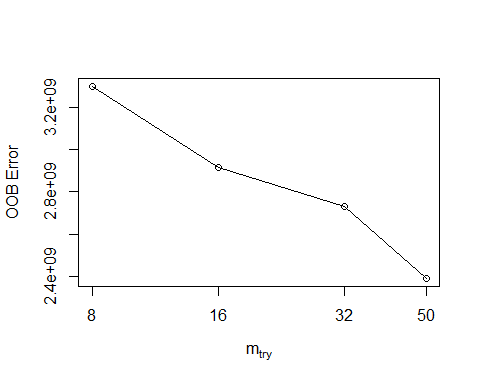
\includegraphics{data_setup_02102019_files/figure-latex/unnamed-chunk-7-1.pdf}

\begin{Shaded}
\begin{Highlighting}[]
\NormalTok{pred <-}\StringTok{ }\KeywordTok{predict}\NormalTok{(}\DataTypeTok{object =} \NormalTok{Mod1, }\DataTypeTok{newdata =} \NormalTok{Wettest)}
\NormalTok{RMSE_Mod1 <-}\StringTok{ }\KeywordTok{rmse}\NormalTok{(}\DataTypeTok{actual =} \NormalTok{Wettest$WetAcres, }\CommentTok{#actual values}
     \DataTypeTok{predicted =} \NormalTok{pred)                       }\CommentTok{#predicted values}
\KeywordTok{print}\NormalTok{(RMSE_Mod1/}\KeywordTok{mean}\NormalTok{(Wettest$WetAcres))      }\CommentTok{#tells us the %of the mean represented by RMSE. AKA "coefficient of variation"}
\end{Highlighting}
\end{Shaded}

\begin{verbatim}
## [1] 0.7512441
\end{verbatim}

\begin{Shaded}
\begin{Highlighting}[]
\CommentTok{# Tune mtry using OOB error}
\KeywordTok{set.seed}\NormalTok{(}\DecValTok{25}\NormalTok{)}
\CommentTok{#train_pred <- predict(object = Mod1, newdata = PAtrain)}
\NormalTok{res <-}\StringTok{ }\KeywordTok{tuneRF}\NormalTok{(}\DataTypeTok{x =} \NormalTok{Wettrain,}
              \DataTypeTok{y =} \NormalTok{Wettrain$WetAcre,}
              \DataTypeTok{ntree =} \DecValTok{500}\NormalTok{,}
              \DataTypeTok{stepfactor =} \FloatTok{0.5}\NormalTok{,}
              \DataTypeTok{doBest=}\OtherTok{TRUE}\NormalTok{,        }\CommentTok{# Returns a random forest model with optimal mtry value}
              \DataTypeTok{importance =} \OtherTok{TRUE}\NormalTok{)}
\end{Highlighting}
\end{Shaded}

\begin{verbatim}
## mtry = 2  OOB error = 104055217 
## Searching left ...
## mtry = 1     OOB error = 665119338 
## -5.391985 0.05 
## Searching right ...
## mtry = 4     OOB error = 2698725 
## 0.9740645 0.05 
## mtry = 6     OOB error = 220350 
## 0.9183503 0.05
\end{verbatim}

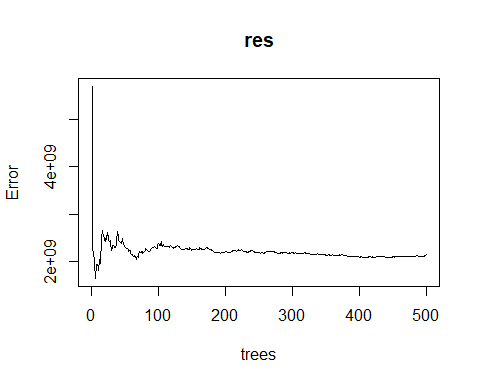
\includegraphics{data_setup_02102019_files/figure-latex/unnamed-chunk-7-2.pdf}

\begin{Shaded}
\begin{Highlighting}[]
              \CommentTok{#localImp = TRUE)}
\KeywordTok{print}\NormalTok{(res)}
\end{Highlighting}
\end{Shaded}

\begin{verbatim}
## 
## Call:
##  randomForest(x = x, y = y, mtry = res[which.min(res[, 2]), 1],      importance = TRUE, stepfactor = 0.5) 
##                Type of random forest: regression
##                      Number of trees: 500
## No. of variables tried at each split: 6
## 
##           Mean of squared residuals: 182323
##                     % Var explained: 99.99
\end{verbatim}

\begin{Shaded}
\begin{Highlighting}[]
\KeywordTok{plot}\NormalTok{(res)}
\end{Highlighting}
\end{Shaded}

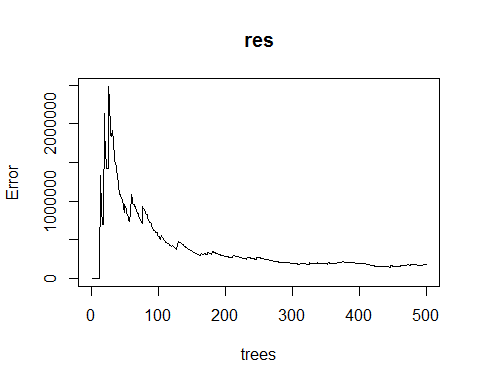
\includegraphics{data_setup_02102019_files/figure-latex/unnamed-chunk-7-3.pdf}

\begin{Shaded}
\begin{Highlighting}[]
\NormalTok{res$importance}
\end{Highlighting}
\end{Shaded}

\begin{verbatim}
##                        %IncMSE IncNodePurity
## Year               234384347.4  1.705639e+10
## month                 128183.8  5.548648e+04
## StateCollege_PRCP    3052427.8  7.795892e+06
## Lebanon_PRCP          115510.7  7.563779e+07
## Selinsgrove_PRCP     -184268.7  1.015508e+07
## WetAcres          6960489329.8  5.724630e+11
\end{verbatim}

\begin{Shaded}
\begin{Highlighting}[]
\KeywordTok{varImpPlot}\NormalTok{(res)                      }
\end{Highlighting}
\end{Shaded}

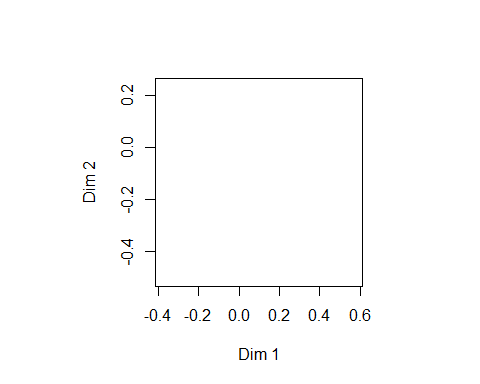
\includegraphics{data_setup_02102019_files/figure-latex/unnamed-chunk-7-4.pdf}

\subsection{Wet Dollars}\label{wet-dollars}

\begin{Shaded}
\begin{Highlighting}[]
\CommentTok{# Split into trainning, validation, and test sets}
\KeywordTok{set.seed}\NormalTok{(}\DecValTok{25}\NormalTok{)}
\NormalTok{assignment <-}\StringTok{ }\KeywordTok{sample}\NormalTok{(}\DecValTok{1}\NormalTok{:}\DecValTok{3}\NormalTok{, }\DataTypeTok{size =} \KeywordTok{nrow}\NormalTok{(WetDollars), }\DataTypeTok{prob =} \KeywordTok{c}\NormalTok{(}\FloatTok{0.7}\NormalTok{, }\FloatTok{0.15}\NormalTok{, }\FloatTok{0.15}\NormalTok{), }\DataTypeTok{replace =} \OtherTok{TRUE}\NormalTok{)}

\NormalTok{Wettrain2 <-}\StringTok{ }\NormalTok{WetDollars[assignment ==}\StringTok{ }\DecValTok{1}\NormalTok{,]}
\NormalTok{Wetvalid2 <-}\StringTok{ }\NormalTok{WetDollars[assignment ==}\StringTok{ }\DecValTok{2}\NormalTok{,]}
\NormalTok{Wettest2 <-}\StringTok{ }\NormalTok{WetDollars[assignment ==}\StringTok{ }\DecValTok{3}\NormalTok{,]}

\KeywordTok{summary}\NormalTok{(Wettrain2)}
\end{Highlighting}
\end{Shaded}

\begin{verbatim}
##       Year          month        StateCollege_PRCP  Lebanon_PRCP   
##  Min.   :2001   Min.   : 1.000   Min.   : 1.620    Min.   : 0.910  
##  1st Qu.:2005   1st Qu.: 4.000   1st Qu.: 5.270    1st Qu.: 6.335  
##  Median :2009   Median : 7.000   Median : 8.050    Median : 9.330  
##  Mean   :2009   Mean   : 6.638   Mean   : 8.831    Mean   : 9.718  
##  3rd Qu.:2014   3rd Qu.:10.000   3rd Qu.:11.370    3rd Qu.:12.145  
##  Max.   :2018   Max.   :12.000   Max.   :26.840    Max.   :39.150  
##  Selinsgrove_PRCP   WetDollars      
##  Min.   : 2.060   Min.   :  129986  
##  1st Qu.: 5.400   1st Qu.: 1653080  
##  Median : 7.920   Median : 7411996  
##  Mean   : 8.842   Mean   : 8099715  
##  3rd Qu.:11.660   3rd Qu.:14673803  
##  Max.   :32.740   Max.   :20514682
\end{verbatim}

\begin{Shaded}
\begin{Highlighting}[]
\KeywordTok{summary}\NormalTok{(Wetvalid2)}
\end{Highlighting}
\end{Shaded}

\begin{verbatim}
##       Year          month        StateCollege_PRCP  Lebanon_PRCP   
##  Min.   :2001   Min.   : 1.000   Min.   : 1.56     Min.   : 1.190  
##  1st Qu.:2007   1st Qu.: 3.000   1st Qu.: 5.99     1st Qu.: 5.692  
##  Median :2012   Median : 6.000   Median : 7.82     Median : 9.090  
##  Mean   :2011   Mean   : 6.077   Mean   : 9.17     Mean   :11.616  
##  3rd Qu.:2015   3rd Qu.: 9.000   3rd Qu.:12.43     3rd Qu.:15.155  
##  Max.   :2018   Max.   :12.000   Max.   :22.57     Max.   :45.690  
##  Selinsgrove_PRCP   WetDollars      
##  Min.   : 0.000   Min.   :  129986  
##  1st Qu.: 5.675   1st Qu.: 1668643  
##  Median : 8.850   Median : 6842246  
##  Mean   :10.449   Mean   : 8398955  
##  3rd Qu.:12.215   3rd Qu.:14673803  
##  Max.   :48.100   Max.   :20011028
\end{verbatim}

\begin{Shaded}
\begin{Highlighting}[]
\KeywordTok{summary}\NormalTok{(Wettest2)}
\end{Highlighting}
\end{Shaded}

\begin{verbatim}
##       Year          month        StateCollege_PRCP  Lebanon_PRCP  
##  Min.   :2002   Min.   : 1.000   Min.   : 2.940    Min.   : 2.31  
##  1st Qu.:2004   1st Qu.: 4.000   1st Qu.: 6.495    1st Qu.: 6.39  
##  Median :2008   Median : 6.000   Median : 9.260    Median :10.04  
##  Mean   :2009   Mean   : 6.074   Mean   : 9.480    Mean   :11.22  
##  3rd Qu.:2014   3rd Qu.: 8.000   3rd Qu.:10.905    3rd Qu.:12.82  
##  Max.   :2018   Max.   :12.000   Max.   :19.730    Max.   :33.07  
##  Selinsgrove_PRCP   WetDollars      
##  Min.   : 0.200   Min.   :  419619  
##  1st Qu.: 5.165   1st Qu.: 1262458  
##  Median : 8.960   Median : 7456851  
##  Mean   : 9.075   Mean   : 8239412  
##  3rd Qu.:11.850   3rd Qu.:11783443  
##  Max.   :26.700   Max.   :20514682
\end{verbatim}

\begin{Shaded}
\begin{Highlighting}[]
\NormalTok{Mod2 <-}\StringTok{ }\KeywordTok{randomForest}\NormalTok{(WetDollars ~}\StringTok{ }\NormalTok{., }
                     \DataTypeTok{data =} \NormalTok{Wettrain2, }
                     \DataTypeTok{ntree =} \DecValTok{500}\NormalTok{, }
                     \CommentTok{#method = "anova", }
                     \DataTypeTok{importance =} \OtherTok{TRUE}\NormalTok{)}

\KeywordTok{print}\NormalTok{(Mod2)                                 }\CommentTok{# % of variance expalined is low. Tuning needed}
\end{Highlighting}
\end{Shaded}

\begin{verbatim}
## 
## Call:
##  randomForest(formula = WetDollars ~ ., data = Wettrain2, ntree = 500,      importance = TRUE) 
##                Type of random forest: regression
##                      Number of trees: 500
## No. of variables tried at each split: 1
## 
##           Mean of squared residuals: 3.843481e+13
##                     % Var explained: 20.23
\end{verbatim}

\begin{Shaded}
\begin{Highlighting}[]
\KeywordTok{summary}\NormalTok{(Mod2)}
\end{Highlighting}
\end{Shaded}

\begin{verbatim}
##                 Length Class  Mode     
## call              5    -none- call     
## type              1    -none- character
## predicted       163    -none- numeric  
## mse             500    -none- numeric  
## rsq             500    -none- numeric  
## oob.times       163    -none- numeric  
## importance       10    -none- numeric  
## importanceSD      5    -none- numeric  
## localImportance   0    -none- NULL     
## proximity         0    -none- NULL     
## ntree             1    -none- numeric  
## mtry              1    -none- numeric  
## forest           11    -none- list     
## coefs             0    -none- NULL     
## y               163    -none- numeric  
## test              0    -none- NULL     
## inbag             0    -none- NULL     
## terms             3    terms  call
\end{verbatim}

\begin{Shaded}
\begin{Highlighting}[]
\KeywordTok{plot}\NormalTok{(Mod2)}
\end{Highlighting}
\end{Shaded}

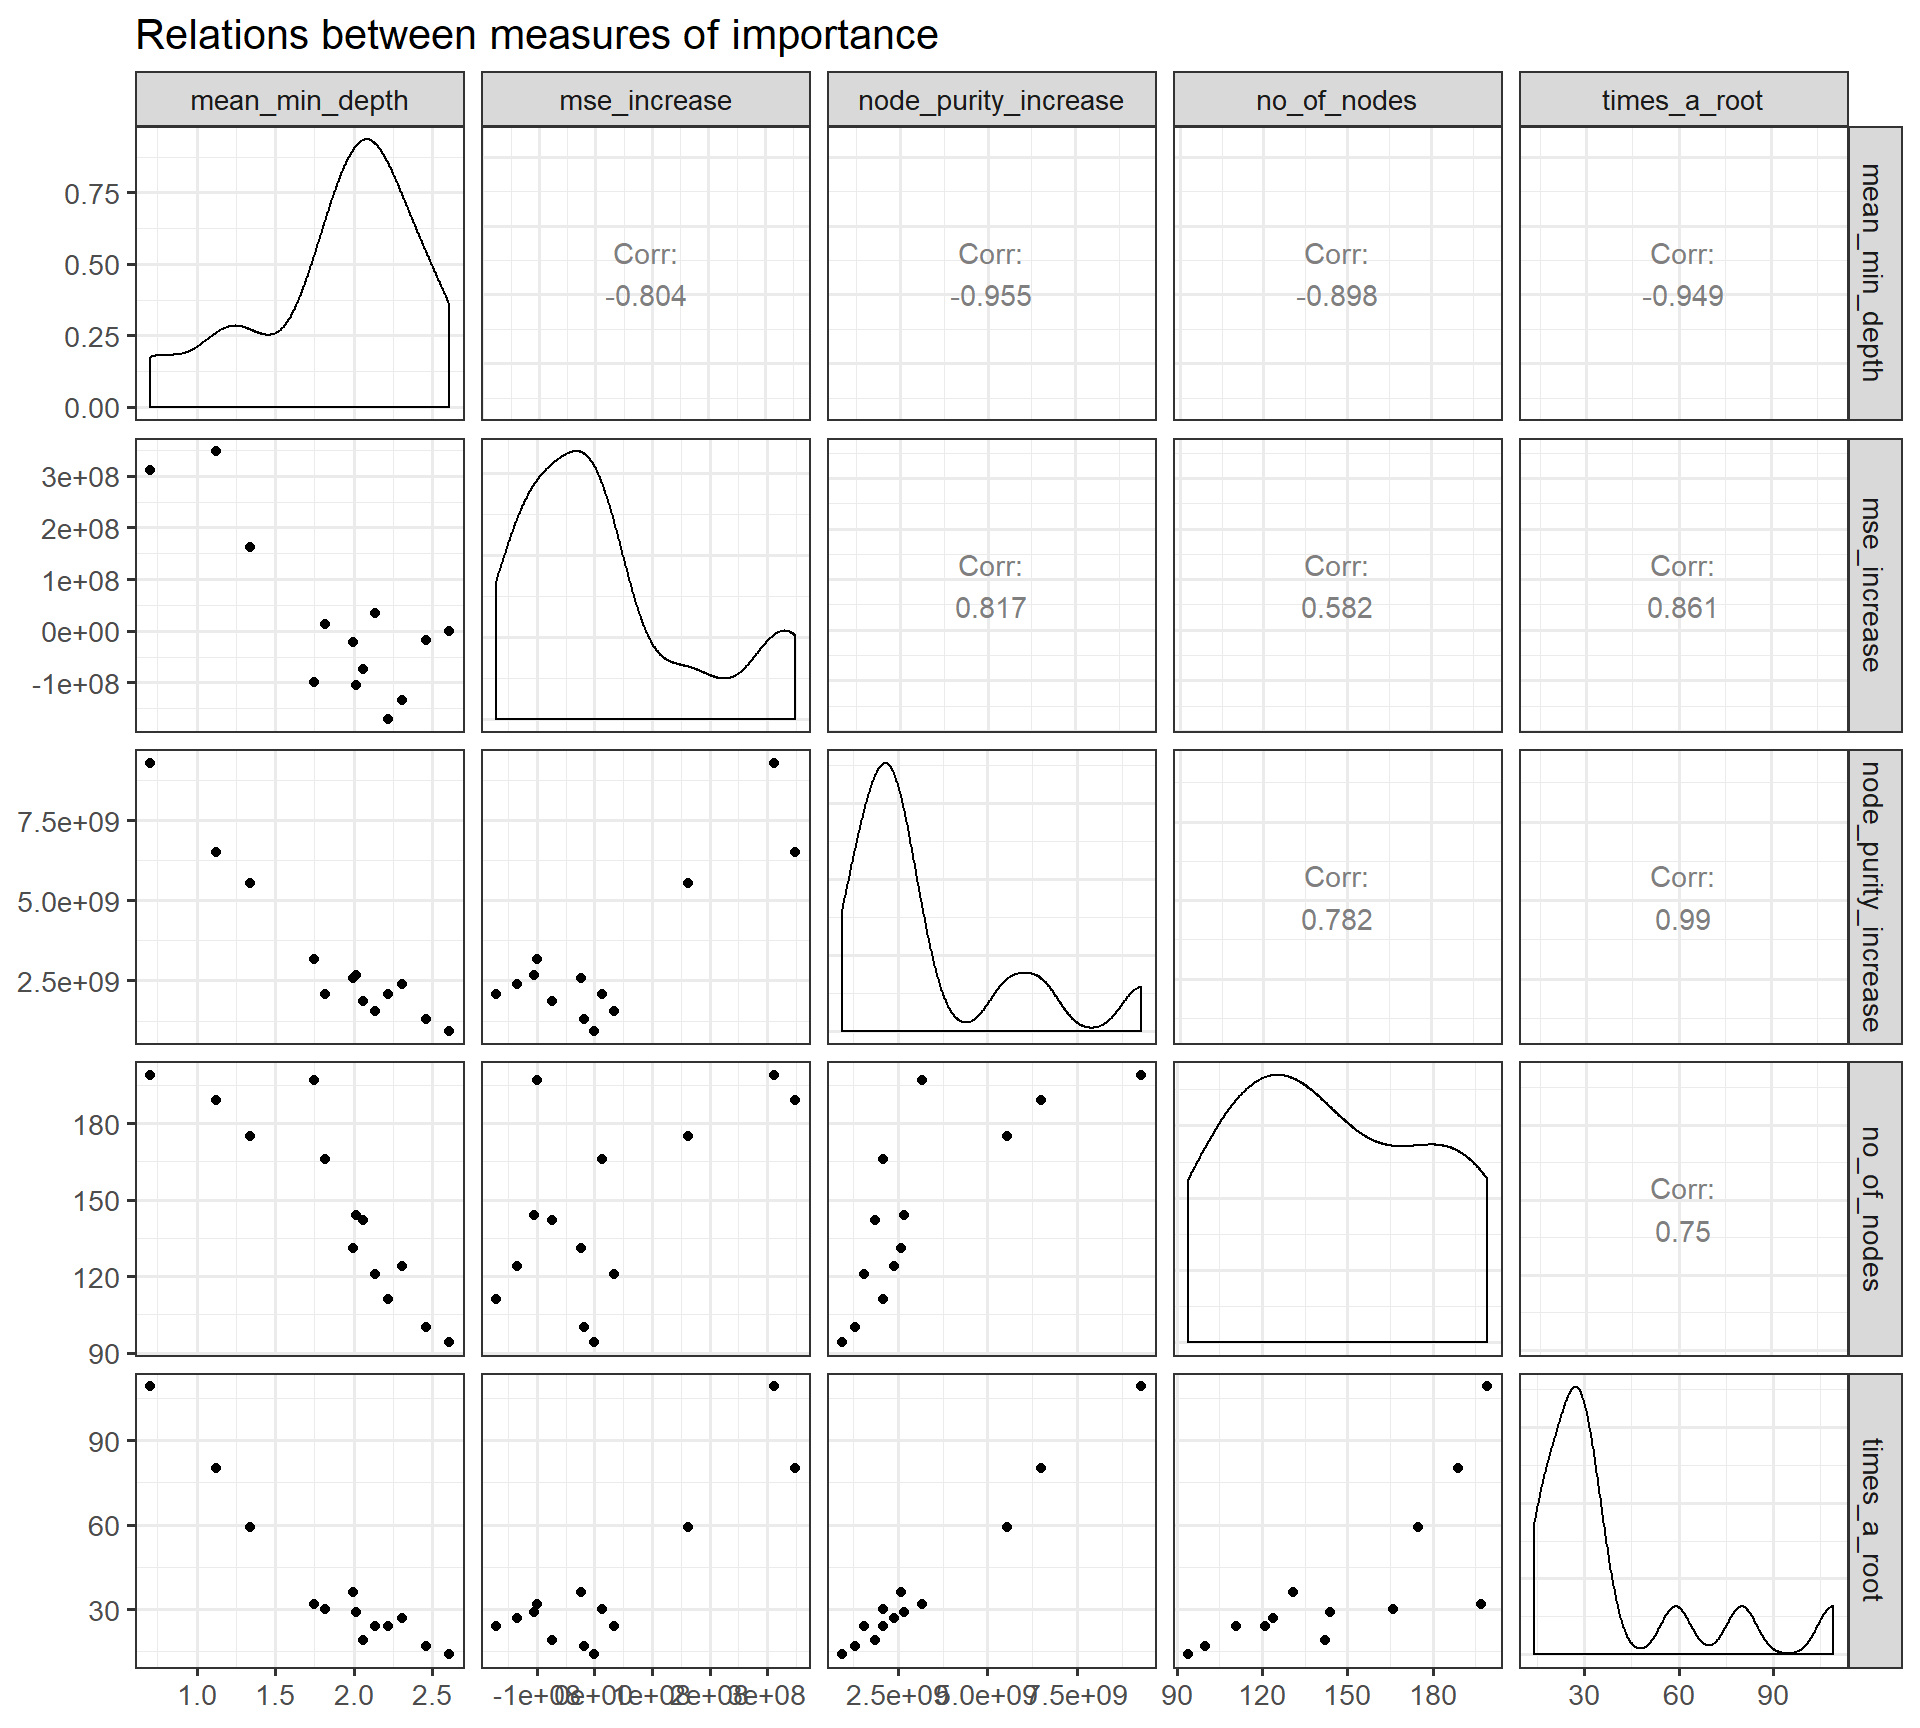
\includegraphics{data_setup_02102019_files/figure-latex/unnamed-chunk-8-1.pdf}

\begin{Shaded}
\begin{Highlighting}[]
\NormalTok{pred2 <-}\StringTok{ }\KeywordTok{predict}\NormalTok{(}\DataTypeTok{object =} \NormalTok{Mod2, }\DataTypeTok{newdata =} \NormalTok{Wettest2)}
\NormalTok{RMSE_Mod2 <-}\StringTok{ }\KeywordTok{rmse}\NormalTok{(}\DataTypeTok{actual =} \NormalTok{Wettest2$WetDollars, }\CommentTok{#actual values}
     \DataTypeTok{predicted =} \NormalTok{pred2)                        }\CommentTok{#predicted values}
\KeywordTok{print}\NormalTok{(RMSE_Mod2/}\KeywordTok{mean}\NormalTok{(Wettest2$WetDollars))      }\CommentTok{#tells us the %of the mean represented by RMSE. AKA "coefficient of variation"}
\end{Highlighting}
\end{Shaded}

\begin{verbatim}
## [1] 0.6656554
\end{verbatim}

\begin{Shaded}
\begin{Highlighting}[]
\CommentTok{# Tune mtry using OOB error}
\KeywordTok{set.seed}\NormalTok{(}\DecValTok{25}\NormalTok{)}
\CommentTok{#train_pred <- predict(object = Mod1, newdata = PAtrain)}
\NormalTok{res2 <-}\StringTok{ }\KeywordTok{tuneRF}\NormalTok{(}\DataTypeTok{x =} \NormalTok{Wettrain2,}
              \DataTypeTok{y =} \NormalTok{Wettrain2$WetDollars,}
              \DataTypeTok{ntree =} \DecValTok{500}\NormalTok{,}
              \DataTypeTok{stepfactor =} \FloatTok{0.5}\NormalTok{,}
              \DataTypeTok{doBest=}\OtherTok{TRUE}\NormalTok{,        }\CommentTok{# Returns a random forest model with optimal mtry value}
              \DataTypeTok{importance =} \OtherTok{TRUE}\NormalTok{)}
\end{Highlighting}
\end{Shaded}

\begin{verbatim}
## mtry = 2  OOB error = 1.099613e+12 
## Searching left ...
## mtry = 1     OOB error = 7.33856e+12 
## -5.673764 0.05 
## Searching right ...
## mtry = 4     OOB error = 16241289456 
## 0.98523 0.05 
## mtry = 6     OOB error = 1715233239 
## 0.8943906 0.05
\end{verbatim}

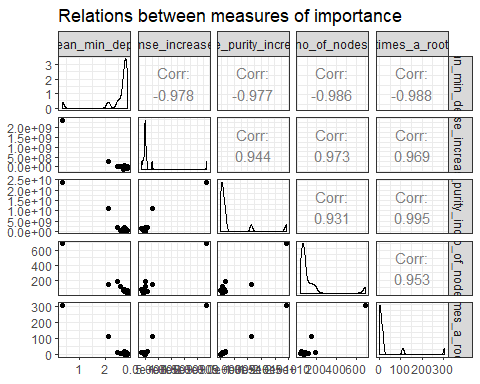
\includegraphics{data_setup_02102019_files/figure-latex/unnamed-chunk-8-2.pdf}

\begin{Shaded}
\begin{Highlighting}[]
              \CommentTok{#localImp = TRUE)}
\KeywordTok{print}\NormalTok{(res2)}
\end{Highlighting}
\end{Shaded}

\begin{verbatim}
## 
## Call:
##  randomForest(x = x, y = y, mtry = res[which.min(res[, 2]), 1],      importance = TRUE, stepfactor = 0.5) 
##                Type of random forest: regression
##                      Number of trees: 500
## No. of variables tried at each split: 6
## 
##           Mean of squared residuals: 1355209009
##                     % Var explained: 100
\end{verbatim}

\begin{Shaded}
\begin{Highlighting}[]
\KeywordTok{plot}\NormalTok{(res2)}
\end{Highlighting}
\end{Shaded}

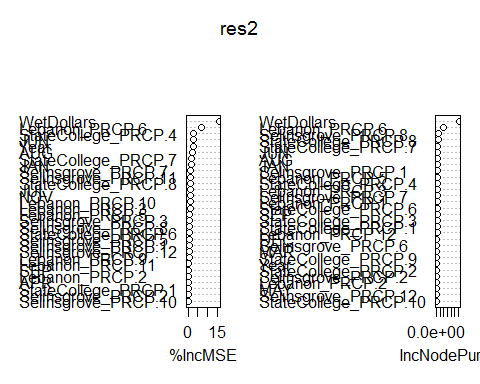
\includegraphics{data_setup_02102019_files/figure-latex/unnamed-chunk-8-3.pdf}

\begin{Shaded}
\begin{Highlighting}[]
\NormalTok{res2$importance}
\end{Highlighting}
\end{Shaded}

\begin{verbatim}
##                         %IncMSE IncNodePurity
## Year               8.579820e+11  6.849186e+13
## month             -3.274544e+10  1.883829e+10
## StateCollege_PRCP  4.678427e+09  2.393336e+10
## Lebanon_PRCP       3.499059e+10  1.863356e+10
## Selinsgrove_PRCP  -8.042994e+09  1.105070e+11
## WetDollars         9.075158e+13  7.776690e+15
\end{verbatim}

\begin{Shaded}
\begin{Highlighting}[]
\KeywordTok{varImpPlot}\NormalTok{(res2)                      }
\end{Highlighting}
\end{Shaded}

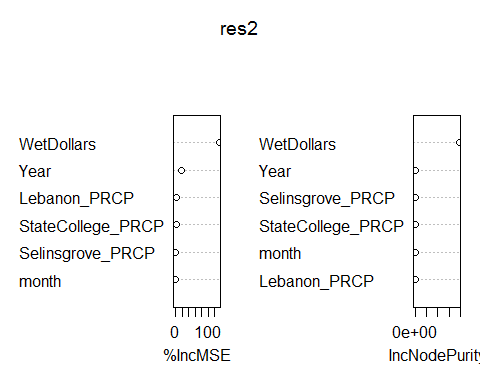
\includegraphics{data_setup_02102019_files/figure-latex/unnamed-chunk-8-4.pdf}
\#\# Dry Acres

\begin{Shaded}
\begin{Highlighting}[]
\CommentTok{# Split into trainning, validation, and test sets}
\KeywordTok{set.seed}\NormalTok{(}\DecValTok{25}\NormalTok{)}
\NormalTok{assignment <-}\StringTok{ }\KeywordTok{sample}\NormalTok{(}\DecValTok{1}\NormalTok{:}\DecValTok{3}\NormalTok{, }\DataTypeTok{size =} \KeywordTok{nrow}\NormalTok{(DryAcres), }\DataTypeTok{prob =} \KeywordTok{c}\NormalTok{(}\FloatTok{0.7}\NormalTok{, }\FloatTok{0.15}\NormalTok{, }\FloatTok{0.15}\NormalTok{), }\DataTypeTok{replace =} \OtherTok{TRUE}\NormalTok{)}

\NormalTok{Drytrain <-}\StringTok{ }\NormalTok{DryAcres[assignment ==}\StringTok{ }\DecValTok{1}\NormalTok{,]}
\NormalTok{Dryvalid <-}\StringTok{ }\NormalTok{DryAcres[assignment ==}\StringTok{ }\DecValTok{2}\NormalTok{,]}
\NormalTok{Drytest <-}\StringTok{ }\NormalTok{DryAcres[assignment ==}\StringTok{ }\DecValTok{3}\NormalTok{,]}

\KeywordTok{summary}\NormalTok{(Drytrain)}
\end{Highlighting}
\end{Shaded}

\begin{verbatim}
##       Year          month        StateCollege_PRCP  Lebanon_PRCP   
##  Min.   :2001   Min.   : 1.000   Min.   : 1.620    Min.   : 0.910  
##  1st Qu.:2005   1st Qu.: 4.000   1st Qu.: 5.270    1st Qu.: 6.335  
##  Median :2009   Median : 7.000   Median : 8.050    Median : 9.330  
##  Mean   :2009   Mean   : 6.638   Mean   : 8.831    Mean   : 9.718  
##  3rd Qu.:2014   3rd Qu.:10.000   3rd Qu.:11.370    3rd Qu.:12.145  
##  Max.   :2018   Max.   :12.000   Max.   :26.840    Max.   :39.150  
##  Selinsgrove_PRCP    DryAcres       
##  Min.   : 2.060   Min.   :   557.8  
##  1st Qu.: 5.400   1st Qu.: 16050.8  
##  Median : 7.920   Median : 80698.0  
##  Mean   : 8.842   Mean   :117531.2  
##  3rd Qu.:11.660   3rd Qu.:174858.0  
##  Max.   :32.740   Max.   :613635.8
\end{verbatim}

\begin{Shaded}
\begin{Highlighting}[]
\KeywordTok{summary}\NormalTok{(Dryvalid)}
\end{Highlighting}
\end{Shaded}

\begin{verbatim}
##       Year          month        StateCollege_PRCP  Lebanon_PRCP   
##  Min.   :2001   Min.   : 1.000   Min.   : 1.56     Min.   : 1.190  
##  1st Qu.:2007   1st Qu.: 3.000   1st Qu.: 5.99     1st Qu.: 5.692  
##  Median :2012   Median : 6.000   Median : 7.82     Median : 9.090  
##  Mean   :2011   Mean   : 6.077   Mean   : 9.17     Mean   :11.616  
##  3rd Qu.:2015   3rd Qu.: 9.000   3rd Qu.:12.43     3rd Qu.:15.155  
##  Max.   :2018   Max.   :12.000   Max.   :22.57     Max.   :45.690  
##  Selinsgrove_PRCP    DryAcres       
##  Min.   : 0.000   Min.   :   557.8  
##  1st Qu.: 5.675   1st Qu.: 19810.8  
##  Median : 8.850   Median : 77513.5  
##  Mean   :10.449   Mean   :115677.5  
##  3rd Qu.:12.215   3rd Qu.:216408.0  
##  Max.   :48.100   Max.   :613635.8
\end{verbatim}

\begin{Shaded}
\begin{Highlighting}[]
\KeywordTok{summary}\NormalTok{(Drytest)}
\end{Highlighting}
\end{Shaded}

\begin{verbatim}
##       Year          month        StateCollege_PRCP  Lebanon_PRCP  
##  Min.   :2002   Min.   : 1.000   Min.   : 2.940    Min.   : 2.31  
##  1st Qu.:2004   1st Qu.: 4.000   1st Qu.: 6.495    1st Qu.: 6.39  
##  Median :2008   Median : 6.000   Median : 9.260    Median :10.04  
##  Mean   :2009   Mean   : 6.074   Mean   : 9.480    Mean   :11.22  
##  3rd Qu.:2014   3rd Qu.: 8.000   3rd Qu.:10.905    3rd Qu.:12.82  
##  Max.   :2018   Max.   :12.000   Max.   :19.730    Max.   :33.07  
##  Selinsgrove_PRCP    DryAcres       
##  Min.   : 0.200   Min.   :   557.8  
##  1st Qu.: 5.165   1st Qu.: 10143.4  
##  Median : 8.960   Median : 74329.0  
##  Mean   : 9.075   Mean   :106350.5  
##  3rd Qu.:11.850   3rd Qu.:136717.0  
##  Max.   :26.700   Max.   :613635.8
\end{verbatim}

\begin{Shaded}
\begin{Highlighting}[]
\NormalTok{Mod3 <-}\StringTok{ }\KeywordTok{randomForest}\NormalTok{(DryAcres ~}\StringTok{ }\NormalTok{., }
                     \DataTypeTok{data =} \NormalTok{Drytrain, }
                     \DataTypeTok{ntree =} \DecValTok{500}\NormalTok{, }
                     \CommentTok{#method = "anova", }
                     \DataTypeTok{importance =} \OtherTok{TRUE}\NormalTok{)}

\KeywordTok{print}\NormalTok{(Mod3)                                 }\CommentTok{# % of variance expalined is low. Tuning needed}
\end{Highlighting}
\end{Shaded}

\begin{verbatim}
## 
## Call:
##  randomForest(formula = DryAcres ~ ., data = Drytrain, ntree = 500,      importance = TRUE) 
##                Type of random forest: regression
##                      Number of trees: 500
## No. of variables tried at each split: 1
## 
##           Mean of squared residuals: 10588143143
##                     % Var explained: 48.68
\end{verbatim}

\begin{Shaded}
\begin{Highlighting}[]
\KeywordTok{summary}\NormalTok{(Mod3)}
\end{Highlighting}
\end{Shaded}

\begin{verbatim}
##                 Length Class  Mode     
## call              5    -none- call     
## type              1    -none- character
## predicted       163    -none- numeric  
## mse             500    -none- numeric  
## rsq             500    -none- numeric  
## oob.times       163    -none- numeric  
## importance       10    -none- numeric  
## importanceSD      5    -none- numeric  
## localImportance   0    -none- NULL     
## proximity         0    -none- NULL     
## ntree             1    -none- numeric  
## mtry              1    -none- numeric  
## forest           11    -none- list     
## coefs             0    -none- NULL     
## y               163    -none- numeric  
## test              0    -none- NULL     
## inbag             0    -none- NULL     
## terms             3    terms  call
\end{verbatim}

\begin{Shaded}
\begin{Highlighting}[]
\KeywordTok{plot}\NormalTok{(Mod3)}
\end{Highlighting}
\end{Shaded}

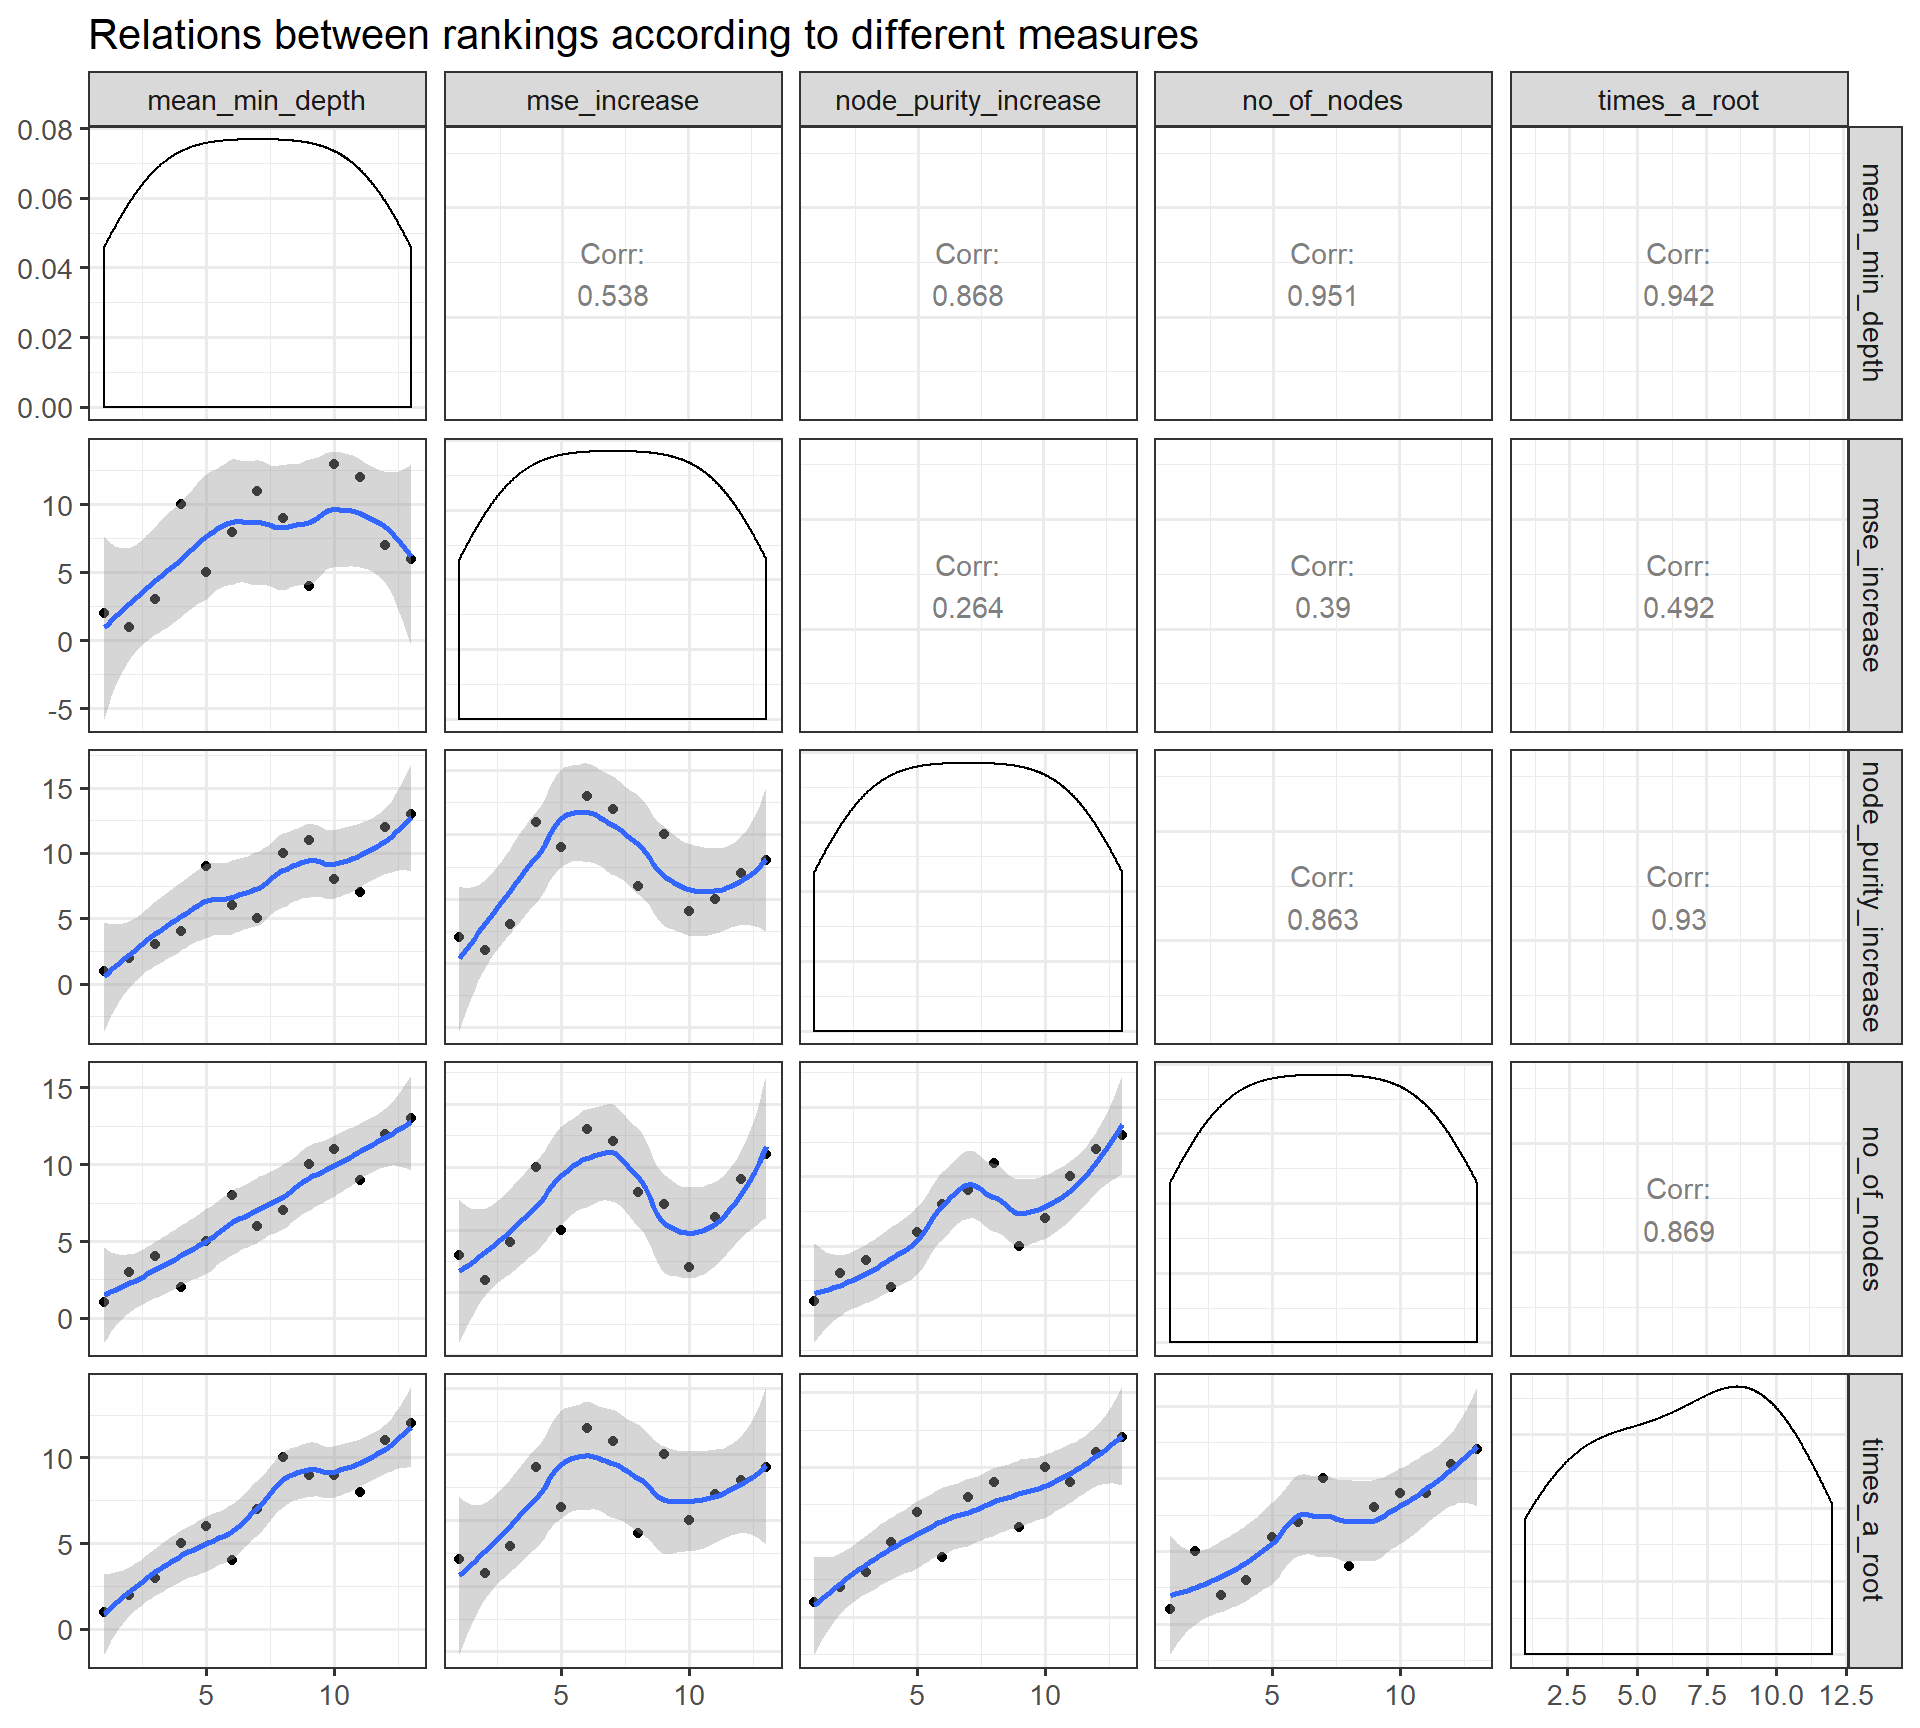
\includegraphics{data_setup_02102019_files/figure-latex/unnamed-chunk-9-1.pdf}

\begin{Shaded}
\begin{Highlighting}[]
\NormalTok{pred3 <-}\StringTok{ }\KeywordTok{predict}\NormalTok{(}\DataTypeTok{object =} \NormalTok{Mod3, }\DataTypeTok{newdata =} \NormalTok{Drytest)}
\NormalTok{RMSE_Mod3 <-}\StringTok{ }\KeywordTok{rmse}\NormalTok{(}\DataTypeTok{actual =} \NormalTok{Drytest$DryAcres, }\CommentTok{#actual values}
     \DataTypeTok{predicted =} \NormalTok{pred3)                        }\CommentTok{#predicted values}
\KeywordTok{print}\NormalTok{(RMSE_Mod3/}\KeywordTok{mean}\NormalTok{(Drytest$DryAcres))      }\CommentTok{#tells us the %of the mean represented by RMSE. AKA "coefficient of variation"}
\end{Highlighting}
\end{Shaded}

\begin{verbatim}
## [1] 1.034596
\end{verbatim}

\begin{Shaded}
\begin{Highlighting}[]
\CommentTok{# Tune mtry using OOB error}
\KeywordTok{set.seed}\NormalTok{(}\DecValTok{25}\NormalTok{)}
\CommentTok{#train_pred <- predict(object = Mod1, newdata = PAtrain)}
\NormalTok{res3 <-}\StringTok{ }\KeywordTok{tuneRF}\NormalTok{(}\DataTypeTok{x =} \NormalTok{Drytrain,}
              \DataTypeTok{y =} \NormalTok{Drytrain$DryAcres,}
              \DataTypeTok{ntree =} \DecValTok{500}\NormalTok{,}
              \DataTypeTok{stepfactor =} \FloatTok{0.5}\NormalTok{,}
              \DataTypeTok{doBest=}\OtherTok{TRUE}\NormalTok{,        }\CommentTok{# Returns a random forest model with optimal mtry value}
              \DataTypeTok{importance =} \OtherTok{TRUE}\NormalTok{)}
\end{Highlighting}
\end{Shaded}

\begin{verbatim}
## mtry = 2  OOB error = 375443571 
## Searching left ...
## mtry = 1     OOB error = 3148461497 
## -7.385978 0.05 
## Searching right ...
## mtry = 4     OOB error = 7126065 
## 0.9810196 0.05 
## mtry = 6     OOB error = 1283593 
## 0.8198736 0.05
\end{verbatim}

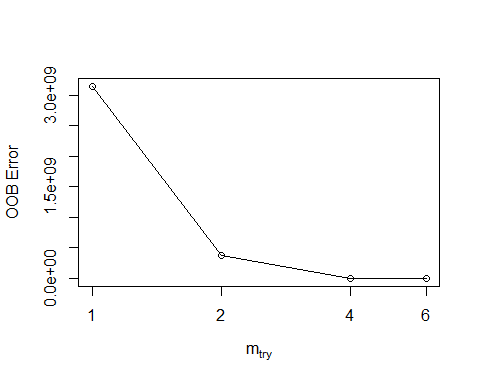
\includegraphics{data_setup_02102019_files/figure-latex/unnamed-chunk-9-2.pdf}

\begin{Shaded}
\begin{Highlighting}[]
              \CommentTok{#localImp = TRUE)}
\KeywordTok{print}\NormalTok{(res3)}
\end{Highlighting}
\end{Shaded}

\begin{verbatim}
## 
## Call:
##  randomForest(x = x, y = y, mtry = res[which.min(res[, 2]), 1],      importance = TRUE, stepfactor = 0.5) 
##                Type of random forest: regression
##                      Number of trees: 500
## No. of variables tried at each split: 6
## 
##           Mean of squared residuals: 344393.2
##                     % Var explained: 100
\end{verbatim}

\begin{Shaded}
\begin{Highlighting}[]
\KeywordTok{plot}\NormalTok{(res3)         }\CommentTok{# looks pretty choppy?}
\end{Highlighting}
\end{Shaded}

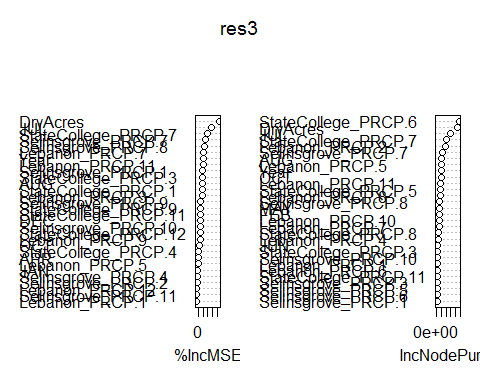
\includegraphics{data_setup_02102019_files/figure-latex/unnamed-chunk-9-3.pdf}

\begin{Shaded}
\begin{Highlighting}[]
\NormalTok{res3$importance}
\end{Highlighting}
\end{Shaded}

\begin{verbatim}
##                         %IncMSE IncNodePurity
## Year               3.408075e+07  2.555319e+09
## month              3.531430e+05  2.042610e+04
## StateCollege_PRCP -5.826061e+04  3.869144e+05
## Lebanon_PRCP       4.122111e+07  1.712351e+07
## Selinsgrove_PRCP   1.101792e+07  1.132820e+06
## DryAcres           4.068888e+10  3.363626e+12
\end{verbatim}

\begin{Shaded}
\begin{Highlighting}[]
\KeywordTok{varImpPlot}\NormalTok{(res3)                      }
\end{Highlighting}
\end{Shaded}

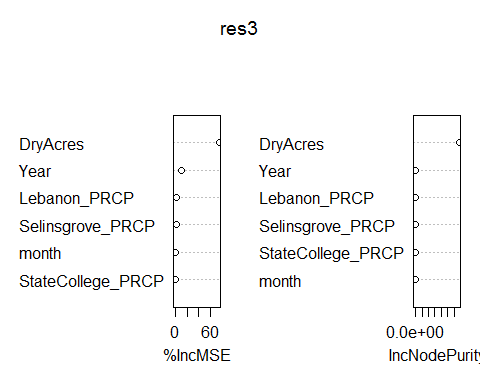
\includegraphics{data_setup_02102019_files/figure-latex/unnamed-chunk-9-4.pdf}

\subsection{Dry Dollars}\label{dry-dollars}

\begin{Shaded}
\begin{Highlighting}[]
\CommentTok{# Split into trainning, validation, and test sets}
\KeywordTok{set.seed}\NormalTok{(}\DecValTok{25}\NormalTok{)}
\NormalTok{assignment <-}\StringTok{ }\KeywordTok{sample}\NormalTok{(}\DecValTok{1}\NormalTok{:}\DecValTok{3}\NormalTok{, }\DataTypeTok{size =} \KeywordTok{nrow}\NormalTok{(DryDollars), }\DataTypeTok{prob =} \KeywordTok{c}\NormalTok{(}\FloatTok{0.7}\NormalTok{, }\FloatTok{0.15}\NormalTok{, }\FloatTok{0.15}\NormalTok{), }\DataTypeTok{replace =} \OtherTok{TRUE}\NormalTok{)}

\NormalTok{Drytrain2 <-}\StringTok{ }\NormalTok{DryDollars[assignment ==}\StringTok{ }\DecValTok{1}\NormalTok{,]}
\NormalTok{Dryvalid2 <-}\StringTok{ }\NormalTok{DryDollars[assignment ==}\StringTok{ }\DecValTok{2}\NormalTok{,]}
\NormalTok{Drytest2 <-}\StringTok{ }\NormalTok{DryDollars[assignment ==}\StringTok{ }\DecValTok{3}\NormalTok{,]}

\KeywordTok{summary}\NormalTok{(Drytrain2)}
\end{Highlighting}
\end{Shaded}

\begin{verbatim}
##       Year          month        StateCollege_PRCP  Lebanon_PRCP   
##  Min.   :2001   Min.   : 1.000   Min.   : 1.620    Min.   : 0.910  
##  1st Qu.:2005   1st Qu.: 4.000   1st Qu.: 5.270    1st Qu.: 6.335  
##  Median :2009   Median : 7.000   Median : 8.050    Median : 9.330  
##  Mean   :2009   Mean   : 6.638   Mean   : 8.831    Mean   : 9.718  
##  3rd Qu.:2014   3rd Qu.:10.000   3rd Qu.:11.370    3rd Qu.:12.145  
##  Max.   :2018   Max.   :12.000   Max.   :26.840    Max.   :39.150  
##  Selinsgrove_PRCP   DryDollars      
##  Min.   : 2.060   Min.   :   77650  
##  1st Qu.: 5.400   1st Qu.: 1592471  
##  Median : 7.920   Median :11030151  
##  Mean   : 8.842   Mean   :12920912  
##  3rd Qu.:11.660   3rd Qu.:17790895  
##  Max.   :32.740   Max.   :54954463
\end{verbatim}

\begin{Shaded}
\begin{Highlighting}[]
\KeywordTok{summary}\NormalTok{(Dryvalid2)}
\end{Highlighting}
\end{Shaded}

\begin{verbatim}
##       Year          month        StateCollege_PRCP  Lebanon_PRCP   
##  Min.   :2001   Min.   : 1.000   Min.   : 1.56     Min.   : 1.190  
##  1st Qu.:2007   1st Qu.: 3.000   1st Qu.: 5.99     1st Qu.: 5.692  
##  Median :2012   Median : 6.000   Median : 7.82     Median : 9.090  
##  Mean   :2011   Mean   : 6.077   Mean   : 9.17     Mean   :11.616  
##  3rd Qu.:2015   3rd Qu.: 9.000   3rd Qu.:12.43     3rd Qu.:15.155  
##  Max.   :2018   Max.   :12.000   Max.   :22.57     Max.   :45.690  
##  Selinsgrove_PRCP   DryDollars      
##  Min.   : 0.000   Min.   :   77650  
##  1st Qu.: 5.675   1st Qu.: 2282997  
##  Median : 8.850   Median : 8585168  
##  Mean   :10.449   Mean   :13427212  
##  3rd Qu.:12.215   3rd Qu.:17790895  
##  Max.   :48.100   Max.   :54954463
\end{verbatim}

\begin{Shaded}
\begin{Highlighting}[]
\KeywordTok{summary}\NormalTok{(Drytest2)}
\end{Highlighting}
\end{Shaded}

\begin{verbatim}
##       Year          month        StateCollege_PRCP  Lebanon_PRCP  
##  Min.   :2002   Min.   : 1.000   Min.   : 2.940    Min.   : 2.31  
##  1st Qu.:2004   1st Qu.: 4.000   1st Qu.: 6.495    1st Qu.: 6.39  
##  Median :2008   Median : 6.000   Median : 9.260    Median :10.04  
##  Mean   :2009   Mean   : 6.074   Mean   : 9.480    Mean   :11.22  
##  3rd Qu.:2014   3rd Qu.: 8.000   3rd Qu.:10.905    3rd Qu.:12.82  
##  Max.   :2018   Max.   :12.000   Max.   :19.730    Max.   :33.07  
##  Selinsgrove_PRCP   DryDollars      
##  Min.   : 0.200   Min.   :   77650  
##  1st Qu.: 5.165   1st Qu.:  986961  
##  Median : 8.960   Median : 5463886  
##  Mean   : 9.075   Mean   :11417461  
##  3rd Qu.:11.850   3rd Qu.:12737743  
##  Max.   :26.700   Max.   :54954463
\end{verbatim}

\begin{Shaded}
\begin{Highlighting}[]
\NormalTok{Mod4 <-}\StringTok{ }\KeywordTok{randomForest}\NormalTok{(DryDollars ~}\StringTok{ }\NormalTok{., }
                     \DataTypeTok{data =} \NormalTok{Drytrain2, }
                     \DataTypeTok{ntree =} \DecValTok{500}\NormalTok{, }
                     \CommentTok{#method = "anova", }
                     \DataTypeTok{importance =} \OtherTok{TRUE}\NormalTok{)}

\KeywordTok{print}\NormalTok{(Mod4)                                 }\CommentTok{# % of variance expalined is low. Tuning needed}
\end{Highlighting}
\end{Shaded}

\begin{verbatim}
## 
## Call:
##  randomForest(formula = DryDollars ~ ., data = Drytrain2, ntree = 500,      importance = TRUE) 
##                Type of random forest: regression
##                      Number of trees: 500
## No. of variables tried at each split: 1
## 
##           Mean of squared residuals: 1.54949e+14
##                     % Var explained: 29.39
\end{verbatim}

\begin{Shaded}
\begin{Highlighting}[]
\KeywordTok{summary}\NormalTok{(Mod4)}
\end{Highlighting}
\end{Shaded}

\begin{verbatim}
##                 Length Class  Mode     
## call              5    -none- call     
## type              1    -none- character
## predicted       163    -none- numeric  
## mse             500    -none- numeric  
## rsq             500    -none- numeric  
## oob.times       163    -none- numeric  
## importance       10    -none- numeric  
## importanceSD      5    -none- numeric  
## localImportance   0    -none- NULL     
## proximity         0    -none- NULL     
## ntree             1    -none- numeric  
## mtry              1    -none- numeric  
## forest           11    -none- list     
## coefs             0    -none- NULL     
## y               163    -none- numeric  
## test              0    -none- NULL     
## inbag             0    -none- NULL     
## terms             3    terms  call
\end{verbatim}

\begin{Shaded}
\begin{Highlighting}[]
\KeywordTok{plot}\NormalTok{(Mod4)}
\end{Highlighting}
\end{Shaded}

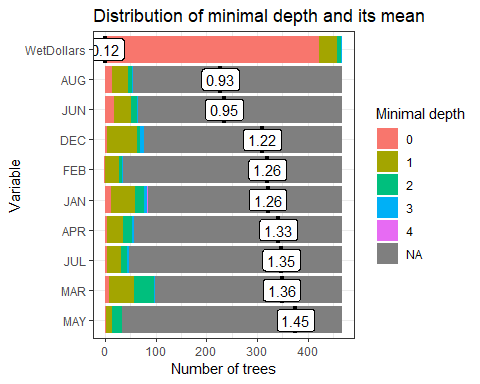
\includegraphics{data_setup_02102019_files/figure-latex/unnamed-chunk-10-1.pdf}

\begin{Shaded}
\begin{Highlighting}[]
\NormalTok{pred4 <-}\StringTok{ }\KeywordTok{predict}\NormalTok{(}\DataTypeTok{object =} \NormalTok{Mod4, }\DataTypeTok{newdata =} \NormalTok{Drytest2)}
\NormalTok{RMSE_Mod4 <-}\StringTok{ }\KeywordTok{rmse}\NormalTok{(}\DataTypeTok{actual =} \NormalTok{Drytest2$DryDollars, }\CommentTok{#actual values}
     \DataTypeTok{predicted =} \NormalTok{pred4)                        }\CommentTok{#predicted values}
\KeywordTok{print}\NormalTok{(RMSE_Mod4/}\KeywordTok{mean}\NormalTok{(Drytest2$DryDollars))      }\CommentTok{#tells us the %of the mean represented by RMSE. AKA "coefficient of variation"}
\end{Highlighting}
\end{Shaded}

\begin{verbatim}
## [1] 1.092932
\end{verbatim}

\begin{Shaded}
\begin{Highlighting}[]
\CommentTok{# Tune mtry using OOB error}
\KeywordTok{set.seed}\NormalTok{(}\DecValTok{25}\NormalTok{)}
\CommentTok{#train_pred <- predict(object = Mod1, newdata = PAtrain)}
\NormalTok{res4 <-}\StringTok{ }\KeywordTok{tuneRF}\NormalTok{(}\DataTypeTok{x =} \NormalTok{Drytrain2,}
              \DataTypeTok{y =} \NormalTok{Drytrain2$DryDollars,}
              \DataTypeTok{ntree =} \DecValTok{500}\NormalTok{,}
              \DataTypeTok{stepfactor =} \FloatTok{0.5}\NormalTok{,}
              \DataTypeTok{doBest=}\OtherTok{TRUE}\NormalTok{,        }\CommentTok{# Returns a random forest model with optimal mtry value}
              \DataTypeTok{importance =} \OtherTok{TRUE}\NormalTok{)}
\end{Highlighting}
\end{Shaded}

\begin{verbatim}
## mtry = 2  OOB error = 6.736511e+12 
## Searching left ...
## mtry = 1     OOB error = 3.753115e+13 
## -4.571304 0.05 
## Searching right ...
## mtry = 4     OOB error = 297907682694 
## 0.9557772 0.05 
## mtry = 6     OOB error = 17967396216 
## 0.939688 0.05
\end{verbatim}

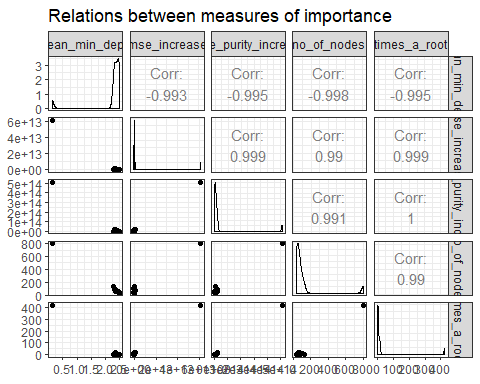
\includegraphics{data_setup_02102019_files/figure-latex/unnamed-chunk-10-2.pdf}

\begin{Shaded}
\begin{Highlighting}[]
              \CommentTok{#localImp = TRUE)}
\KeywordTok{print}\NormalTok{(res4)}
\end{Highlighting}
\end{Shaded}

\begin{verbatim}
## 
## Call:
##  randomForest(x = x, y = y, mtry = res[which.min(res[, 2]), 1],      importance = TRUE, stepfactor = 0.5) 
##                Type of random forest: regression
##                      Number of trees: 500
## No. of variables tried at each split: 6
## 
##           Mean of squared residuals: 9454798682
##                     % Var explained: 100
\end{verbatim}

\begin{Shaded}
\begin{Highlighting}[]
\KeywordTok{plot}\NormalTok{(res4)         }\CommentTok{# looks pretty choppy?}
\end{Highlighting}
\end{Shaded}

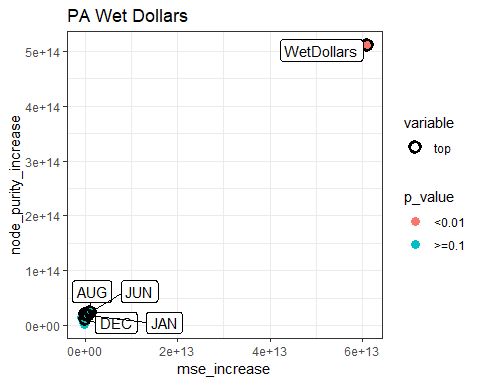
\includegraphics{data_setup_02102019_files/figure-latex/unnamed-chunk-10-3.pdf}

\begin{Shaded}
\begin{Highlighting}[]
\NormalTok{res4$importance}
\end{Highlighting}
\end{Shaded}

\begin{verbatim}
##                         %IncMSE IncNodePurity
## Year               1.713391e+13  1.581166e+15
## month              1.378753e+10  8.809838e+11
## StateCollege_PRCP -1.767504e+11  1.531783e+12
## Lebanon_PRCP       8.771209e+10  2.434308e+10
## Selinsgrove_PRCP   1.089086e+11  1.199370e+11
## DryDollars         4.401359e+14  3.398425e+16
\end{verbatim}

\begin{Shaded}
\begin{Highlighting}[]
\KeywordTok{varImpPlot}\NormalTok{(res4)                      }
\end{Highlighting}
\end{Shaded}

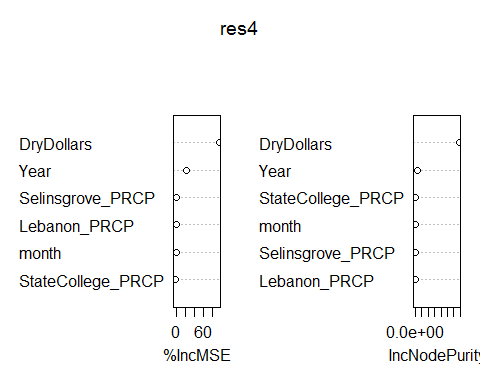
\includegraphics{data_setup_02102019_files/figure-latex/unnamed-chunk-10-4.pdf}

\section{Other optinos for fine tuning the model using control
function}\label{other-optinos-for-fine-tuning-the-model-using-control-function}

\begin{Shaded}
\begin{Highlighting}[]
\NormalTok{Mod2 <-}\StringTok{ }\KeywordTok{randomForest}\NormalTok{(WetAcres ~}\StringTok{ }\NormalTok{., }
                     \DataTypeTok{data =} \NormalTok{Wettrain, }
                     \DataTypeTok{ntree =} \DecValTok{500}\NormalTok{, }
                     \DataTypeTok{mtry =} \DecValTok{6}\NormalTok{,                                        }\CommentTok{# based on tuneRF function results above}
                     \DataTypeTok{importance =} \OtherTok{TRUE}\NormalTok{,}
                     \DataTypeTok{control =} \KeywordTok{rpart.control}\NormalTok{(}\DataTypeTok{minsplit =} \DecValTok{20}\NormalTok{,           }\CommentTok{# default is 20}
                                             \DataTypeTok{cp =} \FloatTok{0.01}\NormalTok{,               }\CommentTok{# default is 0.01}
                                             \DataTypeTok{maxdepth =} \DecValTok{30}\NormalTok{))          }\CommentTok{# default is 30}
\end{Highlighting}
\end{Shaded}

\begin{verbatim}
## Warning in randomForest.default(m, y, ...): invalid mtry: reset to within
## valid range
\end{verbatim}

\begin{Shaded}
\begin{Highlighting}[]
\KeywordTok{print}\NormalTok{(Mod2)}
\end{Highlighting}
\end{Shaded}

\begin{verbatim}
## 
## Call:
##  randomForest(formula = WetAcres ~ ., data = Wettrain, ntree = 500,      mtry = 6, importance = TRUE, control = rpart.control(minsplit = 20,          cp = 0.01, maxdepth = 30)) 
##                Type of random forest: regression
##                      Number of trees: 500
## No. of variables tried at each split: 5
## 
##           Mean of squared residuals: 131875755
##                     % Var explained: 96.37
\end{verbatim}

\begin{Shaded}
\begin{Highlighting}[]
\KeywordTok{summary}\NormalTok{(Mod2)}
\end{Highlighting}
\end{Shaded}

\begin{verbatim}
##                 Length Class  Mode     
## call              7    -none- call     
## type              1    -none- character
## predicted       163    -none- numeric  
## mse             500    -none- numeric  
## rsq             500    -none- numeric  
## oob.times       163    -none- numeric  
## importance       10    -none- numeric  
## importanceSD      5    -none- numeric  
## localImportance   0    -none- NULL     
## proximity         0    -none- NULL     
## ntree             1    -none- numeric  
## mtry              1    -none- numeric  
## forest           11    -none- list     
## coefs             0    -none- NULL     
## y               163    -none- numeric  
## test              0    -none- NULL     
## inbag             0    -none- NULL     
## terms             3    terms  call
\end{verbatim}

\begin{Shaded}
\begin{Highlighting}[]
\KeywordTok{plot}\NormalTok{(Mod2)}
\end{Highlighting}
\end{Shaded}

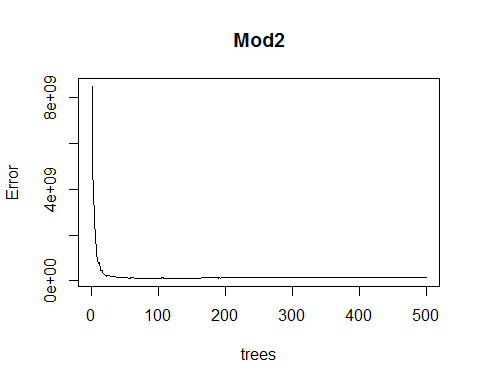
\includegraphics{data_setup_02102019_files/figure-latex/unnamed-chunk-11-1.pdf}

\begin{Shaded}
\begin{Highlighting}[]
\NormalTok{pred <-}\StringTok{ }\KeywordTok{predict}\NormalTok{(}\DataTypeTok{object =} \NormalTok{Mod2, }\DataTypeTok{newdata =} \NormalTok{Wettest)}
\NormalTok{RMSE_Mod2 <-}\StringTok{ }\KeywordTok{rmse}\NormalTok{(}\DataTypeTok{actual =} \NormalTok{Wettest$WetAcres, }\CommentTok{#actual values}
     \DataTypeTok{predicted =} \NormalTok{pred)                       }\CommentTok{#predicted values}
\KeywordTok{print}\NormalTok{(RMSE_Mod2/}\KeywordTok{mean}\NormalTok{(Wettest$WetAcres))      }\CommentTok{#tells us the %of the mean represented by RMSE. AKA "coefficient of variation"}
\end{Highlighting}
\end{Shaded}

\begin{verbatim}
## [1] 0.1633907
\end{verbatim}

\begin{Shaded}
\begin{Highlighting}[]
\CommentTok{#start here in AM}
\CommentTok{#plotcp(Mod2)}
\CommentTok{#summary(rpart(Mod2))}
\end{Highlighting}
\end{Shaded}

\section{Predicting on train set and checking classification
accuracy}\label{predicting-on-train-set-and-checking-classification-accuracy}

\begin{Shaded}
\begin{Highlighting}[]
\CommentTok{#predTrain <- predict(Mod2, PAtrain, type = "class")}
\CommentTok{#table(predTrain, PAtrain$DryAcres)  }
\end{Highlighting}
\end{Shaded}


\end{document}
